\documentclass[12pt,a4paper]{article}
\usepackage{amsmath,amscd,amsbsy,amssymb,latexsym,url,bm,amsthm}
\usepackage{epsfig,graphicx,subfigure}
\usepackage{enumitem,balance}
\usepackage{wrapfig}
\usepackage{here}
\usepackage{mathrsfs,euscript}
\usepackage[usenames]{xcolor}
\usepackage{hyperref}
\usepackage[vlined,ruled,linesnumbered]{algorithm2e}
\usepackage{array}
\hypersetup{colorlinks=true,linkcolor=black}

\newtheorem{theorem}{Theorem}
\newtheorem{lemma}[theorem]{Lemma}
\newtheorem{proposition}[theorem]{Proposition}
\newtheorem{corollary}[theorem]{Corollary}
\newtheorem{exercise}{Exercise}
\newtheorem*{solution}{Solution}
\newtheorem{definition}{Definition}
\theoremstyle{definition}

\renewcommand{\thefootnote}{\fnsymbol{footnote}}

\newcommand{\postscript}[2]
 {\setlength{\epsfxsize}{#2\hsize}
  \centerline{\epsfbox{#1}}}

\renewcommand{\baselinestretch}{1.0}

\setlength{\oddsidemargin}{-0.365in}
\setlength{\evensidemargin}{-0.365in}
\setlength{\topmargin}{-0.3in}
\setlength{\headheight}{0in}
\setlength{\headsep}{0in}
\setlength{\textheight}{10.1in}
\setlength{\textwidth}{7in}
\makeatletter \renewenvironment{proof}[1][Proof] {\par\pushQED{\qed}\normalfont\topsep6\p@\@plus6\p@\relax\trivlist\item[\hskip\labelsep\bfseries#1\@addpunct{.}]\ignorespaces}{\popQED\endtrivlist\@endpefalse} \makeatother
\makeatletter
\renewenvironment{solution}[1][Solution] {\par\pushQED{\qed}\normalfont\topsep6\p@\@plus6\p@\relax\trivlist\item[\hskip\labelsep\bfseries#1\@addpunct{.}]\ignorespaces}{\popQED\endtrivlist\@endpefalse} \makeatother

\begin{document}
\noindent

%========================================================================
\noindent\framebox[\linewidth]{\shortstack[c]{
\Large{\textbf{Lab09-Network Flow}}\vspace{1mm}\\
CS214-Algorithm and Complexity, Xiaofeng Gao \& Lei Wang, Spring 2021.}}
\begin{center}
\footnotesize{\color{red}$*$ If there is any problem, please contact TA Yihao Xie. }

\footnotesize{\color{blue}$*$ Name: BeichenYu  \quad Student ID: 519030910245 \quad Email: polarisybc@sjtu.edu.cn}
\end{center}

\begin{enumerate}
    \item  Consider there is a network consists $n$ computers. For some pairs of computers, a wire $i$ exists in the pair, which means these two computers can communicate with each other. When a signal passes through the wires, the noise in the signal will be amplified. If you know the magnification rate of noise $m_{i,j}$ of each wire (which must be greater than 1). Design an algorithm to find the route  for each other computer to send signals to the computer $v$ with the minimum total magnification rate of noise and analyze the time complexity.
	
	\begin{solution}
		What we need to do is just find a route for each other computer to $ v $, making sure that the product of magnification  rate s along the route is minimal. We can simply take the logarithm of each rate to get a new weight. By denoting $ w_{i,j} = \ln m_{i,j} $, we can change the multiplication problem into an addition problem. Because $ m_{i,j} $ is always greater than 1, we can make sure that all the weights are non-negative. Then, using Dijkstra's Algorithm , we can find a path with the smallest sum of weight for each computer except $ v $, and this is also the route we want. Assume there are $ m $ wires. The calculation of logarithm is $ O(m) $, and the time complexity of Dijkstra's Algorithm is $ O(m+n) $. So the final time complexity is $ O(m+n) $.
	\end{solution}

	\item Suppose that we wish to maintain the transitive closure of a directed graph $G=(V,E)$ as we insert edges into $E$. That is, after each edge has been inserted, we want to update the transitive closure of the edges inserted so far. Assume that the graph $G$ has no edges initially and that we represent the transitive closure as a boolean matrix.
	
	\begin{enumerate}
	    \item Show how to update the transitive closure of a graph $G=(V,E)$ in $O(V^2)$ time when a new edge is added to $G$.
	    \item Give an example of a graph $G$ and an edge $e$ such that $\Omega(V^2)$ time is required to update the transitive closure after the insertion of $e$ into $G$, no matter what algorithm is used.
	    \item Describe an efficient algorithm for updating the transitive closure as edges are inserted into the graph. For any sequence of $m$ insertions, your algorithm should run in total time $\sum_{i=1}^m t_i=O(V^3)$, where $t_i$ is the time to update the transitive closure upon inserting the $i$th edge. Prove that your algorithm attains this time bound.
	\end{enumerate}
	
	\begin{solution}
		\begin{enumerate}
			\item Assume that there are $ n $ vertices in the graph. Denote $ T $ as the transitive closure matrix. If we want to add edge $ (v_{m}, v_{n}) $, we can solve it in $ O(V^2) $ with the algorithm below:\\
			
			First, find the $ n $-th row of $ T $. Record all the number of column that the value of it is 1 in an array $ a_{n} $. Obviously $ \forall i \in a_{n} $, there is a path from $ v_{n} $ to $ v_{i} $.
			
			Second, find the $ m $-th column of $ T $. Record all the number of row that the value of it is 1 in an array $ b_{m} $. Obviously $ \forall i \in b_{m} $, there is a path from $ v_{i} $ to $ v_{m} $.

			Third, for all the $ i \in b_{m} $ and $ j \in a_{n} $, change the value of $ T(i,j) $ into 1.\\

			Because the size of $ a_{n} $ and $ b_{m} $ are both at most $ V $, the time complexity is $ O(V^{2}) $.
			\newpage
			\item The graph is shown below:
				\begin{figure}[H]
				\centering
				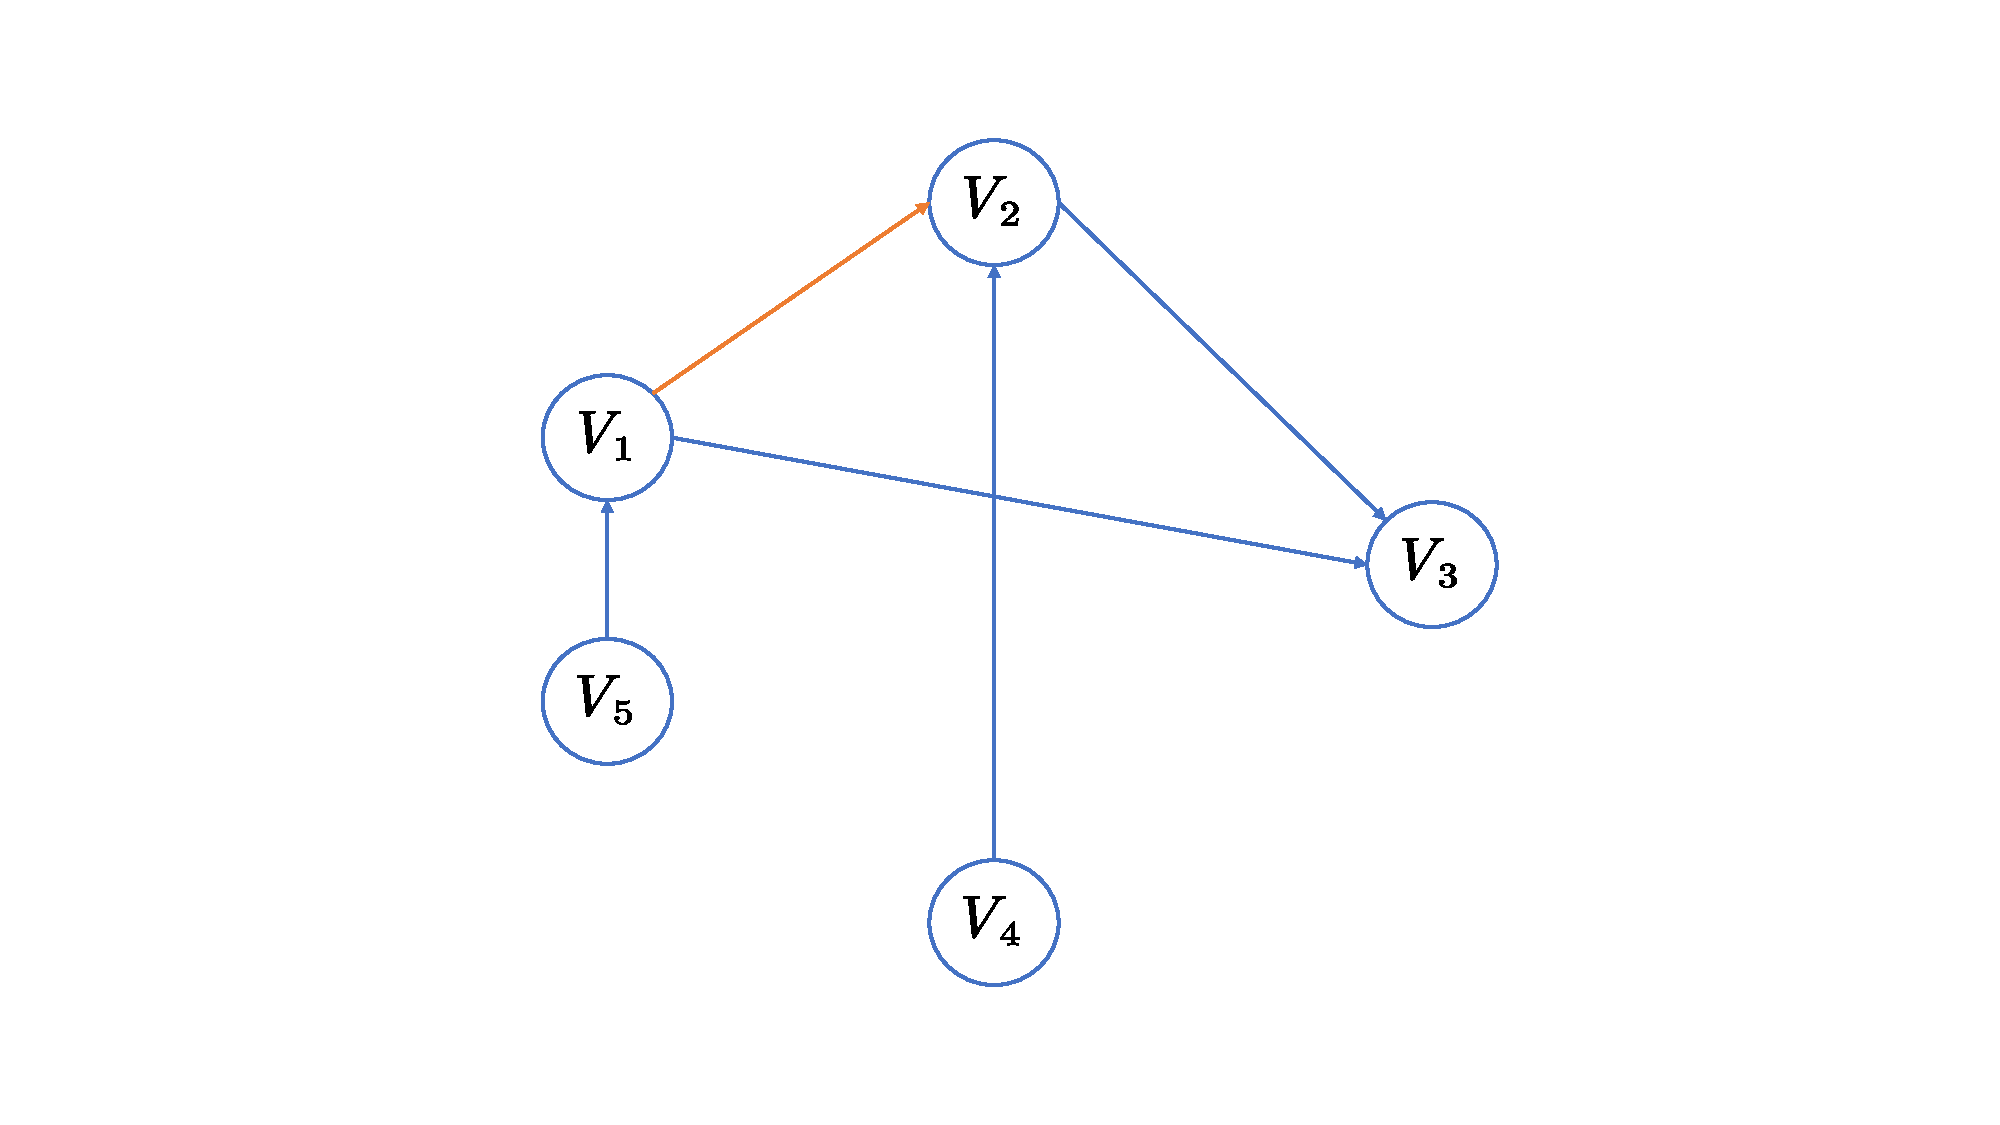
\includegraphics[width=0.8\textwidth]{fig.pdf}
				\caption{Add $ (v_1,v_2) $ to the original directed graph}
				\label{Fig-EscapeProblem}
				\end{figure}
			The original transitive closure matrix is:
			$$ \left[ \begin{array}{ccccc}
				1 & 0 & 1 & 0 & 0\\
				0 & 1 & 1 & 0 & 0\\
				0 & 0 & 1 & 0 & 0\\
				0 & 1 & 1 & 1 & 0\\
				1 & 0 & 1 & 0 & 1 
				\end{array} 
				\right ] $$
			
				According to the algorithm above, we have $ m = 1 $ and $ n = 2 $. So $ a_{2} $ = $ {2,3} $ and $ b_{1} = {1,5} $. So just change $ T(1,2), T(1,3), T(5,2) $ and $ T(5,3) $ into 1. So the result is:

				$$ \left[ \begin{array}{ccccc}
					1 & 1 & 1 & 0 & 0\\
					0 & 1 & 1 & 0 & 0\\
					0 & 0 & 1 & 0 & 0\\
					0 & 1 & 1 & 1 & 0\\
					1 & 1 & 1 & 0 & 1 
					\end{array} 
					\right ] $$
			\item We can just use the Floyd-Warshall Algorithm to solve this problem. Denote $ d_{i,j}$ as the distance from $ v_i $ to $ v_j $. In the beginning, set all  $ d_{i,j} $ to $ \infty $. Then for each edge $ (v_m, v_n) $, set $ d_{m,n} $ to 1. After that, to get the shortest distance from $ v_i $ to $ v_j $, we should check all the vertices $ v_c $. If $ d_{i,c} $ and $ d_{c,j} $ are not all $ \infty $, check whether $ d_{i,c} + d_{c,j} < d_{i,j} $. If it is true, update $ d_{i,j} $ with the value of $ d_{i,c} + d_{c,j} $. 
			
			After all vertices are traversed, if $ d_{i,j} $ is still $ \infty $, we can make sure that there is not a path from $ v_{i} $ to $ v_j $. So finally what we need to do is set $ T(i,j) = 0 $ if $ d_{i,j} = \infty $, and set $ T(i,j) = 1 $ if $ d_{i,j}$ is a finite value.

			Because when checking whether $ d_{i,c} + d_{c,j} < d_{i,j} $ we need to traverse $ v_i , v_j$ and $ v_c $, the time complexity is $ O(V^3) $.


		\end{enumerate}
	\end{solution}

	\item An $n\times n$ grid is an undirected graph consisting of n rows and n columns of vertices, as shown in Figure 26.11. We denote the vertex in the $i$th row and the $j$th column by $(i,j)$. All vertices in a grid have exactly four neighbors, except for the boundary vertices, which are the points $(i,j)$ for which $i = 1, i = n, j = 1$, or $j = n$.
    Given $m\leqslant n^2$ starting points $(x_1,y_1), (x_2, y_2), ... , (x_m, y_m)$ in the grid, the escape problem is to determine whether or not there are $m$ vertex-disjoint paths from the starting points to any $m$ different points on the boundary such that every vertex in $V$ is included in at most one of the $m$ paths. For example, the grid in Figure \ref{Fig-EscapeProblem}(a) has an escape, but the grid in \ref{Fig-EscapeProblem}(b) does not.
    \begin{figure}[!htbp]
	\centering
	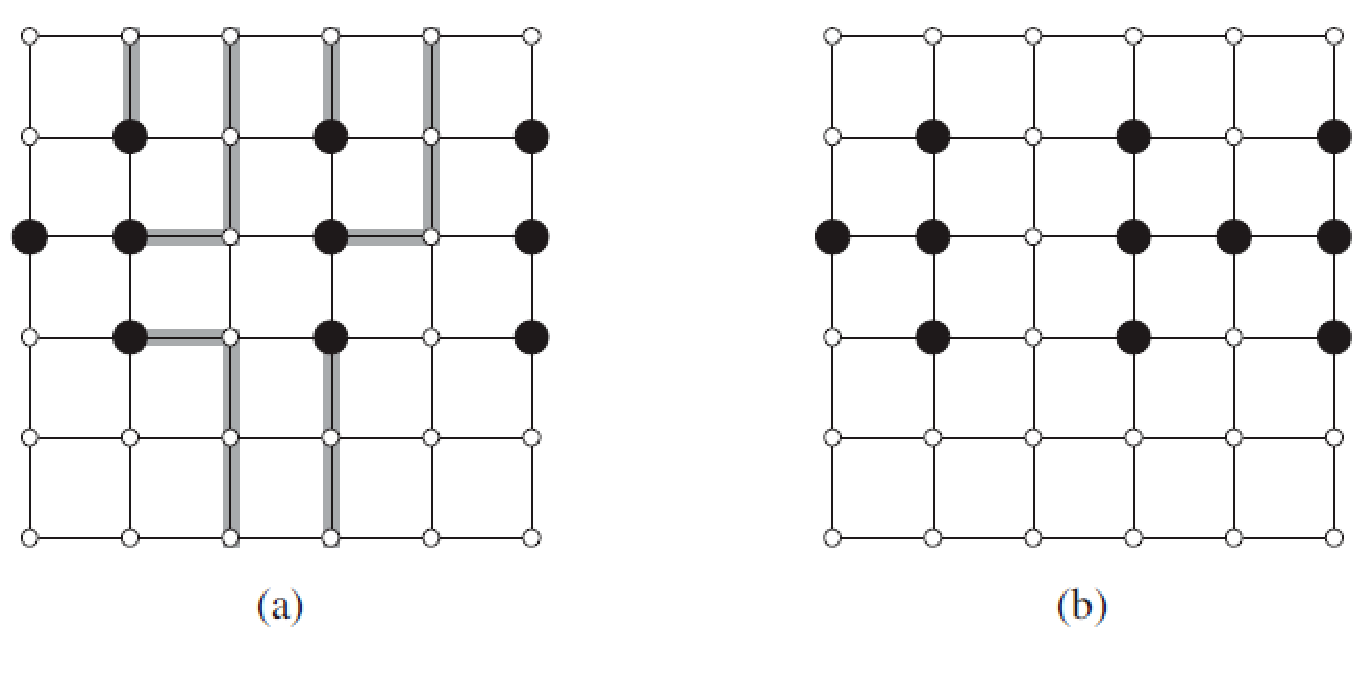
\includegraphics[width=0.5\textwidth]{Fig-EscapeProblem.pdf}
	\caption{Grids for the escape problem. Starting points are black, and other grid vertices are white. (a) A grid with an escape, shown by shaded paths. (b) A grid with no escape.}
	\label{Fig-EscapeProblem}
	\end{figure}
    \begin{enumerate}
        \item Consider a flow network in which vertices, as well as edges, have capacities. That is, the total positive flow entering any given vertex is subject to a capacity constraint. Show that determining the maximum flow in a network with edge and vertex capacities can be reduced to an ordinary maximum-flow problem on a flow network of comparable size. That is, the sizes of the two graph are in the same order of magnitude.
        \item Describe an efficient algorithm to solve the escape problem, and analyze its running time.
    \end{enumerate}
    
	\begin{solution}
		\begin{enumerate}
			\item We can capture the vertex capacities by splitting out each vertex $ v $ into two vertices $ v_{1} $ and $ v_{2} $ ,
			where the capacity of edge $ (v_{1},v_{2}) $ is the vertex capacity of $ v $. If there is an edge $ (u,v) $ in the graph, in the new graph there is an edge $ (u_2, v_1) $ with the same capacity as $ (u,v) $. Then the new flow network will have $ 2|V| $ vertices and $ |V+E| $ edges, which is the same order of magnitude of the original graph.
			
			\item First we need to construct a flow network in which vertices have capacities. For each instruction of grid lines, set a vertex with an unit capacity. For each pair of vertices adjacent in the grid, set a bidirectional  edge with unit capacity. For the $ m $ starting vertices, set an edge of unit capacity from $ s $ to each one; And for all the vertices on the sides, set an edge of unit capacity from each one to $ t $. Using the method above to an ordinary max flow network problem. If the max flow is less then $ m $, then we can conclude that there is no escape in that grid; else the max flow through the network will be the escape path. 
		\end{enumerate}
	\end{solution}
    
\end{enumerate}

\textbf{Remark:} Please include your .pdf, .tex files for uploading with standard file names.
\newpage


%========================================================================
\end{document}